\documentclass[border=1pt]{standalone}
\usepackage{tikz}
\usetikzlibrary{intersections, decorations.pathreplacing}


\begin{document}
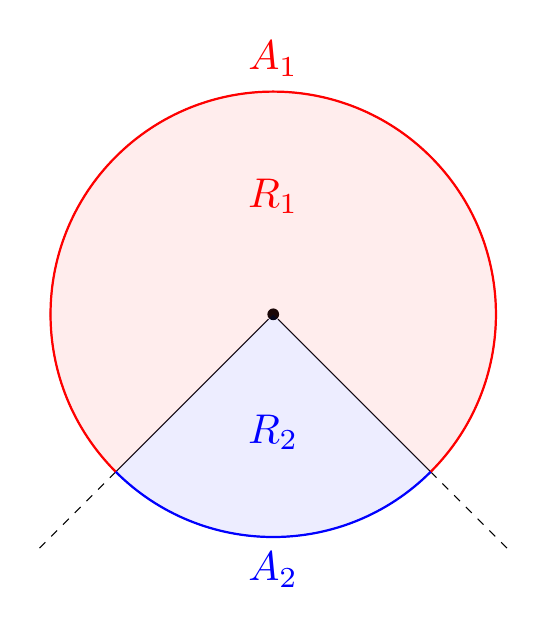
\begin{tikzpicture}[every node/.style={scale=1.5}]
  \node[fill=black, circle, inner sep=1pt] (x) at (0,0) {};

  % Radius of the ball
  \pgfmathsetmacro{\r}{2*sqrt(2)}

  % Draw the circle
  \draw (x) circle (\r);

  % Use a 45-45-90 triangle for the edges
  \coordinate (side1end) at (-2, -2);
  \coordinate (side2end) at (2, -2);

  \draw[name path=side 1] (side1end) -- (x);
  \draw[name path=side 2] (side2end) -- (x);

  % Extend them past our epsilon ball with dotted segments
  \coordinate (side1ext) at (-3, -3);
  \coordinate (side2ext) at (3, -3);

  \draw[dashed] (side1end) -- (side1ext);
  \draw[dashed] (side2end) -- (side2ext);

  \fill[red!70!white, opacity=.1] (side2end) arc (-45:225:\r) -- (0,0)
  -- (side2end);
  \draw[red, thick] (2, -2) arc(-45:225:\r) node[midway, above] {$A_1$};
  \node[red] () at (0, 1.5) {$R_1$};

  \fill[blue!70!white, opacity=.1] (side1end) -- (0,0) -- (side2end)
  arc (315:225:\r) --cycle;
  \draw[blue, thick] (-2, -2) arc(225:315:\r) node[midway, below] {$A_2$};
  \node[blue] () at (0, -1.5) {$R_2$};

  % \draw[blue] (side1end) -- (side2end);




\end{tikzpicture}
\end{document}
